\section{Matrix Limits and Markov Chains} \label{sec 5.3}

\TODOREF{Enhance this bloody hell section when finishing \SEC{7.2}, since the core theorems here depend on that section.}

In this section, we apply what we have learned thus far in \CH{5} to study the \emph{limit} of a sequence of \emph{powers} \(A, A^2, ..., A^n, ...\),
where \(A\) is a square matrix \RED{with \emph{complex} entries}.
(That is, many derived theorems require that the given matrix is over the complex number.)
Such sequences and their limits have practical applications in the natural and social sciences.

\begin{additional definition} \label{adef 5.2}
We \emph{assume familiarity with limits of sequences of real numbers}.
(Refer to some real analysis book.)
The limit of a sequence of \emph{complex} numbers \(\{ z_m : m = 1, 2, ... \}\) can be \emph{defined} in terms of the limits of the sequences of the \emph{real} and \emph{imaginary parts}:
If \(z_m = r_m + \iu s_n\), where \(r_m\) and \(s_m\) are real numbers, and \(\iu\) is the imaginary number such that \(\iu^2 = -1\), then
\[
    \lim_{m \toINF} z_m = \lim_{m \toINF} r_m + \iu \lim_{m \toINF} s_m, 
\]
provided that \(\lim_{m \toINF} r_m\) and \(\lim_{m \toINF} s_m\) exist.
\end{additional definition}

\begin{definition} \label{def 5.10}
Let \(L, A_1, A_2, ...\) be \(n \X p\) matrices having \emph{complex} entries.
The sequence \(A_1, A_2, ...\) is said to \textbf{converge} to the \(n \X p\) matrix \(L\), called the \textbf{limit} of the sequence, if
\[
    \lim_{m \toINF} (A_m)_{ij} = L_{ij}
\]
for all \(1 \le i \le n\) and \(1 \le j \le p\).
To denote that \(L\) is the limit of the sequence, we write
\[
    \lim_{m \toINF} (A_m) = L.
\]
\end{definition}

\begin{note}
這個定義就是把矩陣的極限的存在,reduce 到個別\ entry 的極限的存在,也就是複數\ sequence 的極限的存在;
而根據\ \ADEF{5.2},複數\ sequence 的極限的存在又\ reduce 到(兩個)實數\ sequence 的極限的存在。
然後作者假設讀者知道實數\ sequence 極限存在的定義。
\end{note}

\begin{note}
It seems that calculating limit of sequence of complex numbers require other techniques;
refer to some Complex Analysis course.
\end{note}

\begin{example} \label{example 5.3.1}
If
\[
    A_m = \begin{pmatrix}
        1 - \frac{1}{m} & \left( - \frac{3}{4} \right)^m & \frac{3m^2}{m^2 + 1} + \iu \left( \frac{2m + 1}{m - 1} \right) \\
        \RED{\left( \frac{\iu}{2} \right)^m} & 2 & \left( 1 + \frac{1}{m} \right)^m
    \end{pmatrix}
\]
then by the definition of the limit of sequence of complex numbers, sequence of real numbers, (and Calculus)
\[
    \lim_{m \toINF} A_m = \begin{pmatrix}
        1 & 0 & 3 + 2\iu \\
        0 & 2 & e
    \end{pmatrix},
\]
where \(e\) is the base of the natural algorithm.
\end{example}

\begin{note}
For the red highlight part, see some \href{https://math.stackexchange.com/questions/898296/the-limit-of-complex-sequence}{reference}.
We have
\begin{align*}
    \frac{\abs{\iu}}{\abs{2}} & = \frac{1}{2} & \text{using \DEF{d.3}} \\
        & < 1,
\end{align*}
hence \(\lim_{m \toINF} \left( \cfrac{\abs{\iu}}{\abs{2}} \right)^m = 0\) \MAROON{(1)} \quad by the calculation of sequence of \emph{real} numbers.
And we have
\begin{align*}
    \lim_{m \toINF} \left| \left( \frac{\iu}{2} \right)^m \right|
        & = \lim_{m \toINF} \left( \frac{\abs{\iu}}{\abs{2}} \right)^m & \text{using the solution in the reference} \\
        & = 0 & \text{by \MAROON{(1)}}
\end{align*}
So the absolute value of of the value we want is \(0\), which implies the value we want is also \(0\).
\end{note}

\begin{remark} \label{remark 5.3.1}
A simple, but important, property of matrix limits is contained in the next theorem.
Note the \emph{analogy} with the familiar property of limits of sequences of \emph{real} numbers that asserts that if \(\lim_{m \toINF} a_m\) exists, then
\[
    \lim_{m \toINF} c a_m = c \lim_{m \toINF} a_m.
\]
The next theorem is similar to this fact.
\end{remark}

\begin{theorem} \label{thm 5.11}
Let \(A_1, A_2, ...\) be a sequence of \(n \X p\) matrices with complex entries such the that it converges to the matrix \(L\).
Then for any \(P \in M_{r \X n}(\SET{C})\) and \(Q \in M_{p \X s}(\SET{C})\),
\[
    \lim_{m \toINF} PA_m = P \lim_{m \toINF} A_m = PL \quad \text{ and } \lim_{m \toINF} A_m Q = \left[\lim_{m \toINF} A_m\right] Q = LQ.
\]
\end{theorem}

\begin{proof}
For any \(i (1 \le i \le r)\) and \(j (1 \le j \le p)\),
\begin{align*}
    \lim_{m \toINF} (PA_m)_{ij} & = \lim_{m \toINF} \sum_{k = 1}^n P_{ik} (A_m)_{kj} & \text{by def of matrix multiplication} \\
        & = \sum_{k = 1}^n \lim_{m \toINF} P_{ik} (A_m)_{kj} & \text{change order of limit and summation,} \\
        & & \text{since summation is finite and limit of each term exists} \\
        & = \sum_{k = 1}^n P_{ik} \lim_{m \toINF} (A_m)_{kj} & \text{move ``constant'' out of limit} \\
        & = \sum_{k = 1}^n P_{ik} \cdot L_{kj} & \text{by supposition} \\
        & = (PL)_{ij}. & \text{by def of matrix multiplication}
\end{align*}
Hence \(\lim_{m \toINF} PA_m = PL\).
The proof that \(\lim_{m \toINF} A_m Q = LQ\) is similar.
\end{proof}

\begin{corollary} \label{corollary 5.11.1}
Let \(A \in M_{n \X n}(\SET{C})\) be such that \(\lim_{m \toINF} A^m = L\).
(\(A^m\) is just the \(m\)th power of \(A\).)
Then for any \emph{invertible} matrix \(Q \in M_{n \X n}(\SET{C})\),
\[
    \lim_{m \toINF} (Q A Q^{-1})^m = Q \left[ \lim_{m \toINF} A^m \right] Q^{-1} = Q L Q^{-1}.
\]
\end{corollary}

\begin{proof}
Since
\[
    (Q A Q^{-1})^m = (Q A Q^{-1})(Q A Q^{-1})...(Q A Q^{-1}) = Q A^m Q^{-1},
\]
we have
\begin{align*}
    \lim_{m \toINF} (Q A Q^{-1})^m & = \lim_{m \toINF} Q A^m Q^{-1} & \text{by what we have shown} \\
        & = Q \left[ \lim_{m \toINF} A^m Q^{-1} \right] & \text{by applying \THM{5.11}} \\
        & = Q \left[\lim_{m \toINF} A^m \right] Q^{-1} & \text{by applying \THM{5.11} again} \\
        & = Q L Q.
\end{align*}
\end{proof}

\begin{remark} \label{remark 5.3.2}
In the discussion that follows, we frequently encounter the set
\[
    S = \{ \lambda \in \SET{C}: \abs{\lambda} < 1 or \lambda = 1 \}.
\]
\emph{Geometrically}, this set consists of the complex number \(1\) and the \emph{interior} of the \emph{unit disk}
(the disk of radius \(1\) centered at the origin).
This set is of interest because if \(\lambda\) is a complex number, then \textbf{\(\lim_{m \toINF} \lambda^m\) exists if and only \(\lambda \in S\)}.
This fact, which is obviously true if \(\lambda\) is real, can be shown to be true for complex numbers also.

The following theorem gives \emph{necessary and sufficient conditions} for the existence of the type of limit under consideration.
\end{remark}

\begin{note}
若只看「圓盤」跟實數軸的交集,那個交集內的實數其實也是那些取\ power 後極限存在的實數。
也就是\ \((-1, 1]\) 區間。
\end{note}

\begin{theorem} \label{thm 5.12}
Let \(A\) be a square matrix with complex entries.
Then \(lim_{m \toINF} A^m\) exists if and only if \textbf{both} of the following conditions bold.
\begin{enumerate}
\item Every \emph{eigenvalue} of \(A\) is contained in \(S\) (see \RMK{5.3.2}).
\item If \(1\) is an eigenvalue of \(A\), then the \emph{dimension} of the eigenspace corresponding to \(1\) equals the \emph{algebraic multiplicity} of \(1\) as an eigenvalue of \(A\).
\end{enumerate}
\end{theorem}

\begin{proof}
\RED{Warning: the proof of part(b) needs some other facts in later chapters}.

For part(b), there are two proofs of theorem, but one proof of this theorem, which relies on the theory of \emph{Jordan canonical forms} (\SEC{7.2}), can be found in \EXEC{7.2.19}.
A second proof, which makes use of Schur's theorem (\THM{6.14}), can be found in the article by the author :)

The \textbf{necessity} of condition (a) is easily justified.
For suppose that \(\lambda\) is an eigenvalue of \(A\) such that \(\lambda \RED{\notin} S\).
Let \(v\) be an eigenvector of \(A\) corresponding to \(\lambda\).
Regarding \(v\) as an \(n \X 1\) \emph{matrix}, we see that
\begin{align*}
    \lim_{m \toINF} (A^m v) & = \left( \lim_{m \toINF} A^m \right) v & \text{by \THM{5.11}} \\
        & = Lv,
\end{align*}
where \(L = \lim_{m \toINF} A^m\).
But we also have \(\lim_{m \toINF} (A^mv) = \lim_{m \toINF} \lambda^m v)\) by \EXEC{5.1.16}(b),
but the right side diverges because \(\lim \lambda^m\) does not exist. (Since \(\lambda \notin S\)!)
So \(\lim_{m \toINF} (A^mv)\) does not exist, and we get a contradiction.
So \(\lambda\) must be in \(S\).

Hence if \(\lim_{m \toINF} A^m\) exists, then condition (a) of \THM{5.12} must hold.
\end{proof}

\begin{remark} \label{remark 5.3.3}
Currently, we still cannot prove the \textbf{necessity} of condition (b),
that is, if \(\lim_{m \toINF} A^m\), exists, then condition (a) of \THM{5.12} must hold.

Furthermore, we cannot prove that if condition(a)(b) of \THM{5.12} hold, then \(\lim_{m \toINF} A^m\) exists.

Although we are unable to prove the necessity of condition \((b)\) here, we consider an example such that when (b) fails. then the limit of matrix power does not exist.

Observe that the \CPOLY{} for the matrix
\[
    B = \begin{pmatrix} 1 & 1 \\ 0 & 1 \end{pmatrix}
\]
is \((t - 1)^2\), and hence \(B\) has eigenvalue \(\lambda = 1\) with algebraic multiplicity \(2\).
It can easily be verified that \(\dim(\lambda) = 1\), so that condition (b) of \THM{5.12} is violated.
A simple mathematical induction argument can be used to show that
\[
    B^m = \begin{pmatrix} 1 & m \\ 0 & 1 \end{pmatrix},
\]
and therefore that \(\lim_{m \toINF} B^m\) does not exist.
We see in \CH{7} that if \(A\) is a matrix for which condition (b) \emph{fails}, then \(A\) is \emph{similar to} a matrix whose \emph{upper left \(2 \X 2\) submatrix} is precisely this matrix \(B\).
\end{remark}

In most of the applications involving matrix limits, the matrix is \emph{diagonalizable}, and so (by \THM{5.8}(a),) condition (b) of \THM{5.12} is automatically satisfied.
In this case, \THM{5.12} \emph{reduces to} the following theorem, which can be proved using our previous results.

\begin{theorem} \label{thm 5.13}
Let \(A \in M_{n \X n}(\SET{C})\) satisfy the following two conditions.
\begin{enumerate}
\item[(i)] Every eigenvalue of \(A\) is contained in \(S\) (see \RMK{5.3.2}).
\item \(A\) is diagonalizable.
\end{enumerate}
Then \(\lim_{m \toINF} A^m\) exists.
\end{theorem}

\begin{note}
注意這證明是完全獨立於\ \THM{5.12} 的。
\end{note}

\begin{proof}
Since \(A\) is diagonalizable, there exists an invertible matrix \(Q\) such that \(Q^{-1} A Q = D\) is a diagonal matrix.
(Hence \(A = Q D Q^{-1}\).)
Suppose that
\[
    D = \begin{pmatrix}
        \lambda_1 & 0 & ... & 0 \\
        0 & \lambda_2 & ... & 0 \\
        \vdots & \vdots & & \vdots \\
        0 & 0 & ... & \lambda_n
    \end{pmatrix}.
\]
Because \(\lambda_1, \lambda_2, ... , \lambda_n\) are the eigenvalues of \(A\), condition (i) requires that for each \(i\),
\(\lambda_i \in S\) (see \RMK{5.3.2}), that is, either \(\lambda_i = 1\) or \(\abs{\lambda_i} < 1\).
Thus
\begin{equation*}
    \lim_{m \toINF} \lambda_i^m = \begin{cases}
        1 \quad \text{ if } \lambda_i = 1 \\
        0 \quad \text{ otherwise.}
    \end{cases}
\end{equation*}
But since
\[
    D^m = \begin{pmatrix}
        \lambda_1^m & 0 & ... & 0 \\
        0 & \lambda_2^m & ... & 0 \\
        \vdots & \vdots & & \vdots \\
        0 & 0 & ... & \lambda_n^m
    \end{pmatrix},
\]
the sequence \((D^m)\) converges, and let it converge to \(L\).
Then we have
\begin{align*}
    \lim_{m \toINF} A^m & = \lim_{m \toINF} (Q D Q^{-1})^m & \text{of course} \\
        & = Q L Q^{-1} & \text{by \CORO{5.11.1}}
\end{align*}
\end{proof}

The technique for computing \(\lim_{m \toINF} A^m\) used in the proof of \THM{5.13} can be employed in actual computations, as we now illustrate.
Let
\[
    A = \begin{pmatrix}
        \frac{7}{4} & -\frac{9}{4} & -\frac{15}{4} \\
        \frac{3}{4} & \frac{7}{4}  & \frac{3}{4} \\
        \frac{3}{4} & -\frac{9}{4}  & -\frac{11}{4} \\
    \end{pmatrix}.
\]
Using the methods in \SEC{5.1} and \SEC{5.2}, we obtain
\[
    Q = \begin{pmatrix}
        1 & 3 & -1 \\
        -3 & -2 & 1 \\
        2 & 3 & -1
    \end{pmatrix}
    \quad \text{ and } \quad
    D = \begin{pmatrix}
        1 & 0 & 0 \\
        0 & -\frac{1}{2} & 0 \\
        0 & 0 & \frac{1}{4}
    \end{pmatrix}
\]
such that \(Q^{-1} A Q = D\).
Hence
\begin{align*}
    \lim_{m \toINF} A^m & = \lim_{m \toINF} (Q D Q^{-1})^m = \lim_{m \toINF} Q D^m Q^{-1} = Q (\lim_{m \toINF} D^m) Q^{-1} \\
        & \quad \quad \quad \text{(just the process in the proof of \THM{5.13})} \\
        & = \begin{pmatrix}
                1 & 3 & -1 \\
                -3 & -2 & 1 \\
                2 & 3 & -1
            \end{pmatrix}
            \left[
                \lim_{m \toINF}
                \begin{pmatrix}
                    1 & 0 & 0 \\
                    0 & \left( -\frac{1}{2} \right)^m & 0 \\
                    0 & 0 & \left( \frac{1}{4} \right)^m
                \end{pmatrix}
            \right]
            \begin{pmatrix}
                -1 & 0 & 1 \\
                -1 & 1 & 2 \\
                -5 & 3 & 7
            \end{pmatrix} \\
        & = \begin{pmatrix}
                1 & 3 & -1 \\
                -3 & -2 & 1 \\
                2 & 3 & -1
            \end{pmatrix}
            \begin{pmatrix}
                1 & 0 & 0 \\
                0 & 0 & 0 \\
                0 & 0 & 0
            \end{pmatrix}
            \begin{pmatrix}
                -1 & 0 & 1 \\
                -1 & 1 & 2 \\
                -5 & 3 & 7
            \end{pmatrix} \\
        = \begin{pmatrix}
                -1 & 0 & 1 \\
                3 & 0 & -3 \\
                -2 & 0 & 2
            \end{pmatrix}.
\end{align*}

Next, we consider an application that uses the limit of powers of a matrix.
Suppose that the population of a certain metropolitan area \emph{remains constant} but there is a \emph{continual movement} of people between the city and the suburbs.
Specifically, let the entries of the following matrix \(A\) represent the probabilities that someone living in the city or in the suburbs on January 1 will be living in each region on January 1 \emph{of the next year}.

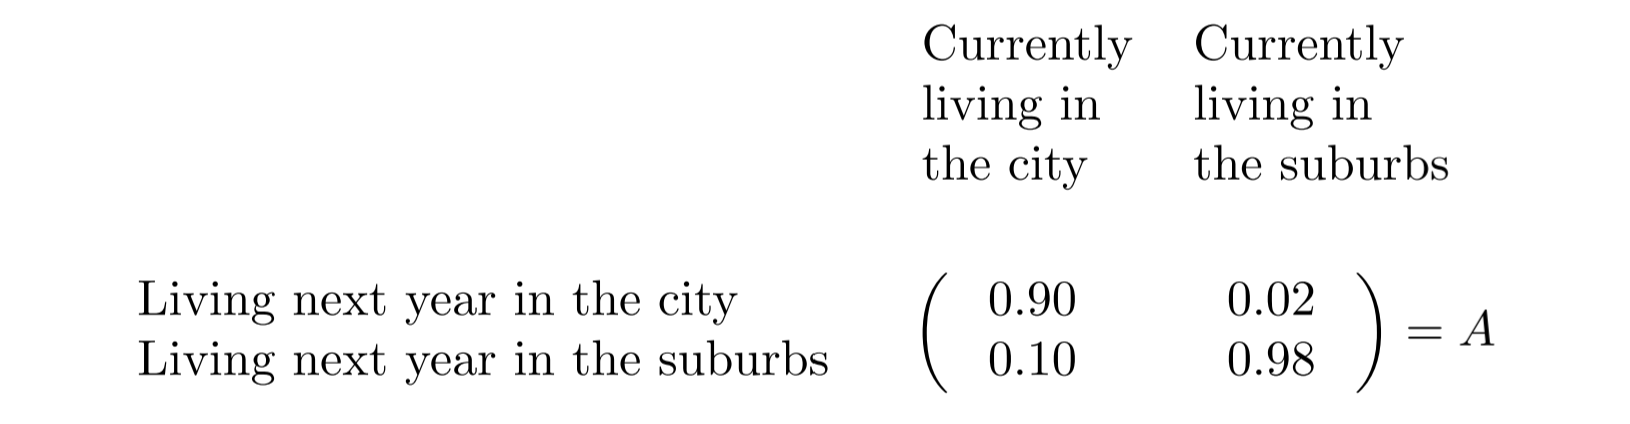
\includegraphics[width=16cm]{images/5-3-city-suburb-movement.png}

For instance, the probability that someone living in the city (on January 1) will be living in the suburbs next year (on January 1) is \(0.10\).
Notice that since the entries of \(A\) are \textbf{probabilities}, they are \textbf{nonnegative}.
Moreover, the \emph{assumption of a constant population} in the metropolitan area requires that \emph{the sum of the entries of each \textbf{column} of \(A\) be \(1\)}.

\begin{additional definition} \label{adef 5.3}
Any square matrix having these two properties (nonnegative entries and columns that sum to \(1\)) is called a \textbf{transition matrix} or a \textbf{stochastic matrix}.
For an arbitrary \(n \X n\) transition matrix \(M\), the rows and columns correspond to \(n\) \textbf{states}, and the entry \(M_{ij}\) represents the probability of moving from state \(j\) to state \(i\) in one \textbf{stage}.
(Note the reversed order of \(ij\)-entry and \(j\)-to-\(i\) movement.)

The \textbf{probability vector} is a vector that has nonnegative entries that sum to \(1\).
Note that each column of a transition matrix is a probability vector.
\end{additional definition}

In our example, there are two states (residing in the city and residing in the suburbs).
So, for example, \(A_{21}\) is the probability of moving from the city to the suburbs in one stage, that is, in one year.
We now determine the probability that a city resident will be living in the suburbs \emph{after \(2\) years}.
There are \emph{two different ways} in which such a move can be made:
remaining in the city for 1 year and then moving to the suburbs, or moving to the suburbs during the first year and remaining there the second year.
(See Figure 5.3.)

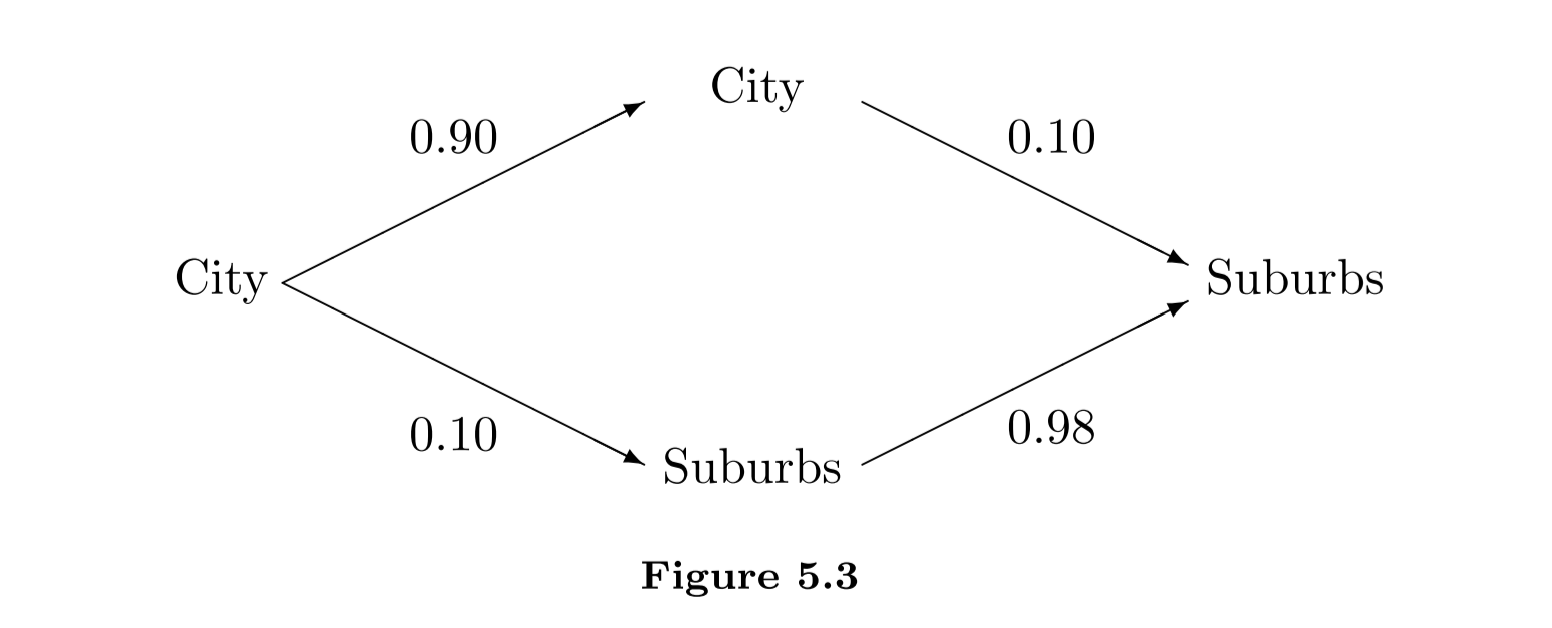
\includegraphics[width=16cm]{images/figure-5-3.png}

The probability that a city dweller remains in the city for the first year is \(0.90\), whereas the probability that the city dweller moves to the suburbs during the first year is \(0.10\).
Hence the probability that a city dweller stays in the city for the first year and then moves to the suburbs during the
second year is the \emph{product} \((0.90)(0.10)\).
Likewise, the probability that a city dweller moves to the suburbs in the first year and remains in the suburbs during the second year is the product \((0.10)(0.98)\).
Thus the probability that a city dweller will be living in the suburbs after 2 years is the \emph{sum of these products}, \((0.90)(0.10) + (0.10)(0.98) = 0.1\).
Observe that this number is \emph{obtained by the same calculation as that which produces \((A^2)_{21}\)},
and hence \((A^2)_{21}\) represents the probability that a city dweller will be living in the suburbs after 2 years.
In general, for any transition matrix \(M\), the entry \((M^m)_{ij}\) represents the probability of moving from state \(j\) to state \(i\) in \(m\) stages.

Suppose additionally that in year 2000, 70\% of the population of the metropolitan area lived in the city and 30\% lived in the suburbs.
We record these data \emph{as a column vector}:

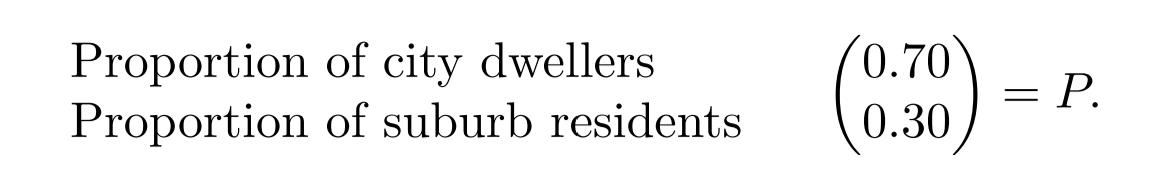
\includegraphics[width=14cm]{images/5-3-city-suburb-prob-vector-1.png}

Notice that the rows of \(P\) correspond to the states of residing in the city and residing in the suburbs, respectively,
and that these \emph{states are listed in the same order as the listing in the transition matrix} \(A\).
Observe also that the column vector \(P\) \emph{contains nonnegative entries that sum to \(1\)};
such a vector is called a \textbf{probability vector}.
In this terminology, \emph{each column of a transition matrix is a probability vector}.
It is often convenient to regard the entries of a transition matrix or a probability vector as \emph{proportions or percentages instead of probabilities}, as we have already done with the probability vector \(P\).

In the vector \(AP = \begin{pmatrix} 0.636 \\ 0.364 \end{pmatrix}\), the first coordinate is the sum \((0.90)(0.70) + (0.02)(0.30)\).
The first term of this sum, \((0.90)(0.70)\), represents the proportion of the 2000 metropolitan population that \emph{remained in the city} during the next year,
and the second term, \((0.02)(0.30)\), represents the proportion of the 2000 metropolitan population that \emph{moved into the city} (from the suburb) during the next year.
Hence the first coordinate of \(AP\) represents the proportion of the metropolitan population that was living in the city in 2001.
Similarly, the second coordinate of \(AP\), represents the proportion of the metropolitan population that was living in the suburbs in 2001.
This argument can be \emph{easily extended} to show that the coordinates of
\[
    A^P = A(AP) = \begin{pmatrix} 0.57968 \\ 0.42032 \end{pmatrix}
\]
represent the proportions of the metropolitan population that were living in each location in 200\RED{2}.
In general, the coordinates of \(A^m P\) represent the \emph{proportion} of the metropolitan population that will be living in the city and suburbs, respectively, after \(m\) stages (\(m\) years after 2000).

From the value of \(AP\) and \(A^2 P\), or just from the value of the entries of \(A\), it seems that the proportion of the population living in cities is getting smaller.
\textbf{Will the city eventually \emph{be depleted} if this trend continues?}
In view of the preceding discussion, it is \emph{natural to define the eventual proportion} of the city dwellers and suburbanites \emph{to be the first and second coordinates, respectively, of} \(\lim_{m \toINF} A^m P\).
We now compute this limit.
It is easily shown that \(A\) is diagonalizable, and so there is an invertible matrix \(Q\) and a diagonal matrix \(D\) such that \(Q^{-1} A Q = D\).
In fact,
\[
    Q = \begin{pmatrix}
        \cfrac{1}{6} & -\cfrac{1}{6} \\ \cfrac{5}{6} & \cfrac{1}{6}
    \end{pmatrix}
    \quad \text{ and }
    D = \begin{pmatrix}
        1 & 0 \\ 0 & 0.88
    \end{pmatrix}.
\]
Therefore (using the process in the proof of \THM{5.13},)
\[
    L = \lim_{m \toINF} A^m = \lim_{m \toINF} Q D^m Q^{-1}) = Q \begin{pmatrix} 1 & 0 \\ 0 & 0 \end{pmatrix} Q^{-1} =
    \begin{pmatrix}
        \cfrac{1}{6} & \cfrac{1}{6} \\ \cfrac{5}{6} & \cfrac{5}{6}
    \end{pmatrix}
\]
Consequently, (by \THM{5.11})
\[
    \lim_{m \toINF} A^m P = LP = \begin{pmatrix}
        \cfrac{1}{6} \\ \cfrac{5}{6}
    \end{pmatrix}
\]
Thus, eventually, \(\frac{1}{6}\) of the population will live in the city and \(\frac{5}{6}\) will live in the suburbs each year.
Note that the vector \(LP\) satisfies \(A (LP) = LP  = 1 \cdot LP\).
Hence \(LP\) is \textbf{both a probability vector} and \textbf{an eigenvector of \(A\)} corresponding \textbf{to the eigenvalue \(1\)}. Since the eigenspace of \(A\) corresponding to the eigenvalue \(1\) is one-dimensional (just by calculation),
there is only one such vector \(L\), that is, the vector that is an eigenvector of \(A\) corresponding to the eigenvalue \(1\) and sums its entries to \(1\) is \emph{unique}.
And \(LP\) is \textbf{independent of the initial choice} of probability vector \(P\).
(See \EXEC{5.3.15}.)
For example, had the 2000 metropolitan population consisted entirely of city dwellers, the
limiting outcome would be the same.

\begin{remark} \label{remark 5.3.4}
In analyzing the city suburb problem, we gave \emph{probabilistic interpretations} of \(A^2\) and \(AP\), showing that \(A^2\) is a transition matrix and \(AP\) is a probability vector.
In fact, the product of any two transition matrices \emph{is} a transition matrix, and the product of any transition matrix and probability vector \emph{is} a probability vector.
A proof of these facts is a simple corollary of the next theorem, which characterizes transition matrices and probability
vectors.
\end{remark}

\begin{theorem} \label{thm 5.14}
Let \(M\) be an \(n \X n\) matrix having \emph{real nonnegative} entries, let \(v\) be a column vector in \(\SET{R}^n\) having nonnegative coordinates, and let \(u \in \SET{R}^n\) be the column vector in which \emph{each coordinate equals \(1\)}.
Then
\begin{enumerate}
\item \(M\) is a transition matrix if and only if \(u^\top M = u^\top\);
\item \(v\) is a probability vector if and only if \(u^\top v = (1)\).
\end{enumerate}
\end{theorem}

\begin{proof}
See \EXEC{5.3.16}.
\end{proof}

\begin{corollary} \label{corollary 5.14.1} \ 

\begin{enumerate}
\item The product of two \(n \X n\) transition matrices is an \(n \X n\) transition matrix.
In particular, any power of a transition matrix is a transition matrix.

\item The product of a transition matrix and a probability vector is a probability vector.
\end{enumerate}
\end{corollary}

\begin{proof}
See \EXEC{5.3.16}.
\end{proof}

\begin{remark} \label{remark 5.3.5}
The city-suburb problem is \emph{an example of a process} in which elements of a set are each \emph{classified as being in one of several fixed states} that \emph{can switch over time}.
In general, such a process is called a \textbf{stochastic process}.
The switching to a particular state is described by a probability, and \emph{in the most general case}, this probability depends on such factors as the state in question, the \emph{time} in question, some or all of the \emph{previous states} in which the object has been (including the current state), and the states that \emph{other objects} are in or have been in.

(For instance, the object could be an American voter, and the state of the object could be his or her preference of political party.
In this example, all four of the factors mentioned above influence the probability that an object is in a particular state at a particular time.)

If, however, the probability that an object in one state \(A\) changes to a different state \(B\) \emph{in a fixed interval of time} depends only on the two states \(A\) and \(B\) (and not on the time, earlier states, or other factors), then the stochastic process is called a \textbf{Markov process}.
If, in addition, the number of possible states is \emph{finite}, then the Markov process is called a \textbf{Markov chain}.
We treated the city suburb example as a two-state Markov chain.
Of course, a Markov process is usually only an idealization of reality because the probabilities involved are almost never constant over time.

Note that some literature defines Markov chain as a Markov process and having \emph{countable} states.
\end{remark}

(Skip another example in page 290 to 292.)

In the preceding two examples, we saw that \(\lim_{m \toINF} A^m P\), where \(A\) is the transition matrix and \(P\) is the initial probability vector of the Markov chain, gives the eventual proportions in each state.
In general, however, \textbf{the limit of powers of a transition matrix need not exist}.
For example, if
\[
    M = \begin{pmatrix} 0 & 1 \\ 1 & 0 \end{pmatrix},
\]
then \(\lim_{m \toINF} M^m\) does not exist because odd powers of \(M\) equal \(M\) and even powers of \(M\) equal \(I\).
The reason that the limit fails to exist is that \textbf{condition (a) of \THM{5.12} does not hold for \(M\)} (\(-1\) is an eigenvalue, but \(-1 \notin S\) where \(S\) is defined in \RMK{5.3.2}).
In fact, it can be shown (see \EXEC{7.2.20}) that \textbf{the only transition matrices} \(A\) such that \(\lim_{m \toINF} A^m\) does not exist are precisely those matrices for which condition (a) of \THM{5.12} fails to hold.

But even if the limit of powers of the transition matrix exists, the computation of the limit may be quite difficult.
(The reader is encouraged to work \EXEC{5.3.6} to appreciate the truth of the last sentence.)
Fortunately, there is a large and important class of transition matrices for which this limit exists and is easily computed -- this is the class of \textbf{regular transition matrices}.

\begin{definition} \label{def 5.11}
A transition matrix is called \textbf{regular} if \emph{some power} of the matrix contains only nonzero (i.e., positive) entries.
\end{definition}

\begin{example} \label{example 5.3.2}
The transition matrix
\[
    \begin{pmatrix} 0.90 & 0.02 \\ 0.10 & 0.98 \end{pmatrix}
\]
of the Markov chain used in the city-suburb problem is clearly regular because each entry is positive.
On the other hand, the transition matrix
\[
    A = \begin{pmatrix}
        1 & 0.4 & 0.1 & 0 \\
        0 & 0.3 & 0.5 & 0 \\
        0 & 0 & 0.2 & 0 \\
        0 & 0.3 & 0.2 & 1
    \end{pmatrix}
\]
is not regular because the first column of \(A^m\) is
\[
    \begin{pmatrix} 1 \\ 0 \\ 0 \\ 0 \end{pmatrix}
\]
for any power \(m\).

Observe that a regular transition matrix \emph{may contain zero entries}.
For example,
\[
    M = \begin{pmatrix} 0.9 & 0.5 & 0 \\ 0 & 0.5 & 0.4 \\ 0.1 & 0 & 0.6 \end{pmatrix}
\]
is regular because every entry of \(M^2\) is positive.
\end{example}

\begin{remark} \label{remark 5.3.6}
The remainder of this section is devoted to proving that, for a \textbf{regular} transition matrix \(A\), the \emph{limit} of the sequence of powers of \(A\) exists and \textbf{has identical columns}.
From this fact, it is easy to compute this limit.
In the course of proving this result, we \emph{obtain some interesting bounds for the magnitudes of eigenvalues of any square matrix}.
These bounds are given in terms of the sum of the absolute values of the rows and columns of the matrix.
The necessary terminology is introduced in the definitions that follow.
\end{remark}

\begin{definition} \label{def 5.12}
Let \(A \in M_{n \X n}(\SET{C})\).
For \(1 \le i, j \le n\), define \(\rho_i(A)\) to be the sum of the \emph{absolute values} of the entries of row \(i\) of \(A\), and define \(\nu(A)\) to be equal to the sum of the absolute values of the entries of column \(j\) of \(A\).
Thus
\[
    \rho_i(A) = \sum_{j = 1}^n \abs{A_{ij}} \quad \text{for} i = 1, 2, ..., n
\]
and
\[
    \nu_j(A) = \sum_{i = 1}^n \abs{A_{ij}} \quad \text{for} j = 1, 2, ..., n.
\]
The \textbf{row sum} of \(A\), denoted \(\rho(A)\), and the \textbf{column sum} of \(A\), denoted \(\nu(A)\), are defined as
\[
    \rho(A) = \max \{ \rho_i(A) : 1 \le i \le n \} \quad \text{ and } \quad \nu(A) = \max \{ \nu_j(A) : 1 \le j \le n \}.
\]
\end{definition}

\begin{example} \label{example 5.3.3}
For the matrix
\[
    A = \begin{pmatrix}
        1 & -\iu & 3-4\iu \\
        -2+\iu & 0 & 6 \\
        3 & 2 & \iu
    \end{pmatrix}
\]
\(\rho_1(A) = 7, \rho_2(A) = 6 + \sqrt{5}, \rho_3(A) = 6, \nu_1(A) = 4 + \sqrt{5}, \nu_2(A) = 3\), and  \(\nu_3(A) = 12\).
Hence \(\rho(A) = 6 + \sqrt{5}\) and \(\nu(A) = 12\).
\end{example}

Our next results show that the \emph{smaller} of \(\rho(A)\) and \(\nu(A)\) is an \textbf{upper bound for the absolute values of eigenvalues of \(A\).} 
In the preceding example, for instance, \(A\) has no eigenvalue with absolute value greater than \(6 + \sqrt{5}\).

To obtain a \emph{geometric view} of the following theorem, we introduce some terminology.
\begin{additional definition}
For an \(n \X n\) matrix \(A\), we define the \(i\)th \textbf{Gershgorin disk} \(C_i\) to be the \emph{disk in the complex plane} with center \(A_{ii}\) and radius \(r_i = \rho_i(A) - \abs{A_{ii}}\);
that is
\[
    C_i = \{ z \in \SET{C} : \abs{z - A_{ii}} \le r_i \}.
\]
\end{additional definition}

For example, consider the matrix
\[
    A = \begin{pmatrix} 1 + 2 \iu & 1 \\ 2 \iu & -3 \end{pmatrix}.
\]
For this matrix, \(C_1\) is the disk with center \(1 + 2\iu\) and radius \(1\), and \(C_2\) is the disk with center \(-3\) and radius \(2\).
(See Figure 5.4)

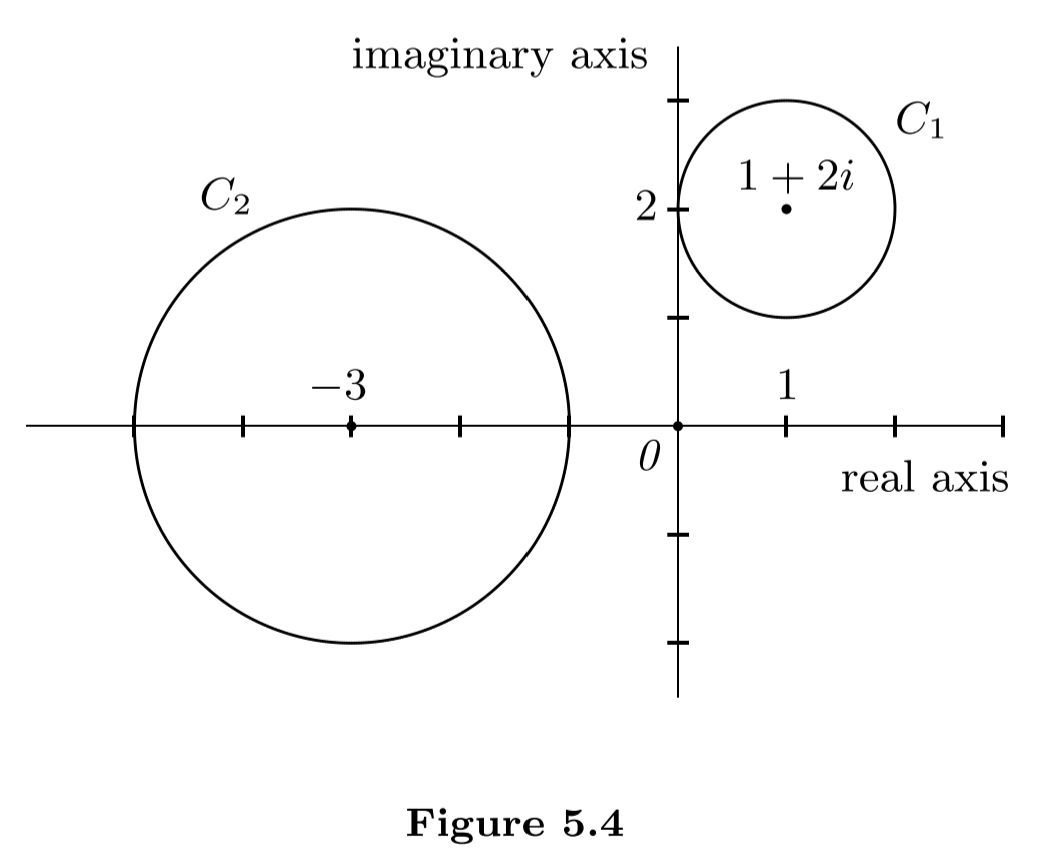
\includegraphics[width=14cm]{images/figure-5-4.png}

Gershgorin's circle theorem, stated below, tells us that all the eigenvalues of \(A\) are located within these two disks.
In particular, we see that \(0\) is \emph{not} an eigenvalue, and hence by \EXEC{5.1.9}(c), \(A\) is invertible.

\begin{theorem} [Gershgorin's Circle Theorem] \label{thm 5.15}
Let \(A \in M_{n \X n}(\SET{C})\).
Then every eigenvalue of \(A\) is contained in a Gersbgorin disk.
\end{theorem}

\begin{proof}
Let \(\lambda\) be an eigenvalue of \(A\) with the corresponding eigenvector
\[
    v = \begin{pmatrix} v_1 \\ v_2 \\ \vdots \\ v_n \end{pmatrix}.
\]
Then \(v\) satisfies the matrix equation \(Av = \lambda v\), which can be written as
\[
    \sum_{j = 1}^n A_{ij} v_j = \lambda v_i \text{for \(1 \le i \le n\)}. \quad \quad \quad \MAROON{(1)}
\]
Suppose that \(v_k\) is a coordinate of \(v\) having the \emph{largest absolute value}; \MAROON{(2)} \quad \quad
note that since \(v\) is an eigenvector, \(v \ne \OV\), hence some coordinate \(v_i\) is nonzero, which implies \(v_k \ne 0\). \MAROON{(3)} \quad \quad
We show that \(\lambda\) \textbf{lies in \(C_k\)}, that is, \(\abs{\lambda - A_{kk}} \le r_k\).
(We will do some trick: multiply \(\abs{v_k}\) in the both sides of this to-be-proved inequality.)
For \(i = k\), it follows from \(\MAROON{(1)}\) that
\begin{align*}
    \abs{v_k}\abs{\lambda - A_{kk}} & = \abs{(v_k)(\lambda - A_{kk})} & \text{by \THM{d.3}(a)} \\
        & = \abs{\lambda v_k - A_{kk} v_k} & \text{of course} \\
        & = \left| \sum_{j = 1}^n A_{kj} v_j - A_{kk} v_k \right| & \text{by \MAROON{(1)}} \\
        & = \left| \sum_{j \ne k} A_{kj} v_j \right| & \text{of course} \\
        & \le \sum_{j \ne k} \abs{ A_{kj} } \abs{ v_j } & \text{by \THM{d.3}(c)} \\
        & \le \sum_{j \ne k} \abs{ A_{kj} } \abs{ v_{\RED{k}} } & \text{by \MAROON{(2)}} \\
        & = \abs{v_k} \sum_{j \ne k} \abs { A_{kj} } & \text{move ``constant'' out of summation} \\
        & = \abs{v_k} r_k. & \text{by def of \(r_k\)}
\end{align*}
Thus we have \(\abs{v_k}\abs{\lambda - A_{kk}} \le \abs{v_k} r_k\).
And since by \MAROON{(3)}, \(\abs{v_k} > 0\), hence (by cancellation law) we have \(\abs{\lambda - A_{kk}} \le r_k\).
\end{proof}

\begin{corollary} \label{corollary 5.15.1}
Let \(\lambda\) be any eigenvalue of \(A \in M_{n \X n}(\SET{C})\).
Then \(\abs{lambda} \le \rho(A)\).
\end{corollary}

\begin{proof}
By Gershgorin's circle theorem, \(\abs{\lambda - A_{kk}} \le r_k\) for some \(k\). \MAROON{(1)} \quad \quad
Hence
\begin{align*}
    \abs{\lambda} & = \abs{(\lambda - A_{kk}) + A_{kk}} & \text{of course} \\
        & \le \abs{\lambda - A_{kk}} + \abs{A_{kk}} & \text{by \THM{d.3}(c)} \\
        & \le r_k + \abs{A_{kk}} & \text{by \MAROON{(1)}} \\
        & = \rho_k(A) & \text{by \DEF{5.12}} \\
        & \le \rho(A). & \text{by definition}
\end{align*}
\end{proof}

\begin{note}
這個\ Corollary 的意義是,eigenvalue 的絕對值會小於等於矩陣的行和。
\end{note}

\begin{corollary} \label{corollary 5.15.2}
Let \(\lambda\) be any eigenvalue of \(A \in M_{n \X n}(\SET{C})\).
Then
\[
    \abs{\lambda} \le \min \{ \rho(A), \nu(A) \}.
\]
\end{corollary}

\begin{proof}
Since \(\abs{\lambda} \le \rho(A)\) by \(1\), it suffices to show that \(\abs{\lambda} \le \nu(A)\).
By \EXEC{5.1.15}, \(\lambda\) is an eigenvalue of \(A^\top\), and so \(\abs{\lambda} \le \rho(A^\top)\) by \CORO{5.15.1}.
But the rows of \(A^\top\) are the columns of \(A\); consequently \(\rho(A^\top) = \nu(A)\).
Therefore \(\abs{\lambda} \nu(A)\).
\end{proof}

The next corollary is immediate from \CORO{5.15.2}
\begin{corollary} \label{corollary 5.15.3}
If \(\lambda\) is an eigenvalue of a \emph{transition} matrix, then \(\abs{\lambda} \le 1\).
(Since each column of a transition matrix sums to \(1\).)
\end{corollary}

\begin{theorem} \label{thm 5.16}
Every \emph{transition} matrix has \(1\) as an eigenvalue.
\end{theorem}

\begin{proof}
Let \(A\) be an \(n \X n\) \emph{transition} matrix, and let \(u \in \SET{R}^n\) be the column vector in which \emph{each coordinate is \(1\)}.
Then \(A^\top u = u\) by \THM{5.14}, and hen\(c\)e \(u\) is an eigenvector of \(A^\top\) corresponding to the eigenvalue \(1\). But since \(A\) and \(A^\top\) have the same eigenvalues, it follows that \(1\) is also an eigenvalue of \(A\).
\end{proof}

Suppose that \(A\) is a transition matrix for which some eigenvector corresponding to the eigenvalue \(1\) \emph{has only nonnegative coordinates}.
Then some multiple of this vector is \emph{a probability vector} \(P\) as well as an eigenvector of \(A\) corresponding to eigenvalue \(1\).
It is interesting to \emph{observe}(i.e. not proved yet) that if \(P\) is the initial probability vector of a Markov chain having \(A\) as its transition matrix, then the Markov chain is \emph{completely static}.
(That is, in particular, \(AP = P\).)
For in this situation, \(A^m P = P\) for every positive integer \(m\); hence the probability of being in each state never
changes.
Consider, for instance, the city suburb problem with
\[
    P = \begin{pmatrix} \cfrac{1}{6} \\ \cfrac{5}{6} \end{pmatrix}.
\]

\begin{theorem} \label{thm 5.17}
Let \(A \in M_{n \X n}(\SET{C})\) be a matrix in which each entry is a positive real number, and let \(\lambda\) be a \emph{complex} eigenvalue of \(A\) such that \(\abs{\lambda} = \rho(A)\).
Then \(\lambda = \rho(A)\) and \(\{ u \}\) is a basis for \(E_{\lambda}\), where \(u \in C^n\) is the column vector in which each coordinate equals \(1\).
\end{theorem}

\begin{note}
That is, given a ``positive'' matrix \(A\), if \(\lambda\) is an eigenvalue and equal to the row sum of \(A\), then \(\lambda\) is in fact also positive.
\end{note}

\begin{proof}
Let \(v\) be an \emph{arbitrary} eigenvector of \(A\) corresponding to \(\lambda\), with coordinates \(v_1, v_2, ..., v_n\).
Suppose that \(v_k\) is the coordinate of \(v\) having the \emph{largest absolute value}, and let \(b = \abs{v_k}\). \MAROON{(b.0)}

Then
\begin{align*}
    \rho(A) b & = \abs{\lambda} b & \text{by supposition} \\
        & = \abs{\lambda} \abs{v_k} & \text{by \MAROON{(b.0)}} \\
        & = \abs{\lambda v_k} & \text{by \THM{d.3}(a)} \\
        & = \left| \sum_{j = 1}^n A_{kj} v_j \right| & \text{in particular from the fact \(Av = \lambda v\)} \\
        &\ \RED{\le} \sum_{j = 1}^n \abs{ A_{kj} v_j } & \text{by \THM{d.3}(c)} \\
        & = \sum_{j = 1}^n \abs{A_{kj}} \abs{v_j} & \text{by \THM{d.3}(a)} \\
        &\ \RED{\le} \sum_{j = 1}^n \abs{A_{kj}} \abs{v_{\RED{k}}} = \sum_{j = 1}^n \abs{A_{kj}} b & \text{since \(\abs{v_k}\) is the largest and \MAROON{(b.0)}} \\
        & = \rho_k(A) b & \text{by def of \(\rho_k(A)\)} \\
        &\ \RED{\le} \rho(A) b \quad \quad \quad \MAROON{(1)} & \text{by def of \(\rho(A)\)}.
\end{align*}
So the three inequalities in the derivation above are actually equalities; that is,
\begin{enumerate}
\item \(\left| \sum_{j = 1}^n A_{kj} v_j \right| \RED{=} \sum_{j = 1}^n \abs{ A_{kj} v_j }\),
\item \(\sum_{j = 1}^n \abs{A_{kj}} \abs{v_j} \RED{=} \sum_{j = 1}^n \abs{A_{kj}} b\), and
\item \(\rho_k(A) b \RED{=} \rho(A)\).
\end{enumerate}

We will see in \EXEC{6.1.15}(b) that (a) holds if and only if all the terms \(A_{kj} v_j (j = 1, 2, ... , n)\) are obtained by multiplying some nonzero complex number \(z\) by nonnegative \textbf{real} numbers.
(That is, intuitively, (a) holds, if and only if all these complex numbers are \textbf{parallel and have same direction} in the complex plane.)
Without loss of generality, we assume that \(\abs{z} = 1\). \MAROON{(b.2)}
Thus there exist nonnegative real numbers \(c_1, c_2, ..., c_n\) such that
\[
    A_{kj} v_j = c_j z. \quad \quad \quad \MAROON{(2)}
\]
By (b) and the assumption (that each entry is a positive real number, so) that \(A_{kj} \ne 0\) for all \(k\) and \(j\), we have
\[
    \abs{v_j} = \abs{v_k} = b \text{ for } j = 1, 2, ..., n. \quad \quad \quad \MAROON{(3)}
\]

%根據假設,所有 \(\abs{v_j}\) 都小於等於 \(\abs{v_k}\)。若這時真的有一個 \(\abs{v_j}\) 是 "小於" \(\abs{v_k}\),則 \(\sum_{j = 1}^k \abs{v_j}\) 就一定小於 \(\sum_{j = 1}^n \abs{v_k} = \sum_{j = 1}^n b\)。連帶的,(b) 會是錯的,矛盾。

Combining \MAROON{(2)} and \MAROON{(3)}, we obtain that for \(j = 1, 2, ..., n\),
\begin{align*}
    b & = \abs{v_k} & \text{by \MAROON{(b.0)}} \\
      & = \left| \frac{c_j}{A_{kj}} z \right| & \text{by \MAROON{(2)}}\\
      & = \left| \frac{c_j}{A_{kj}} \right| \abs{z} = \left| \frac{c_j}{A_{kj}} \right| & \text{by \MAROON{(b.2)}} \\
      & = \frac{c_j}{A_{kj}}, & \text{since \(c_j, A_{kj}\) are nonnegative}
\end{align*}
and therefore, by \MAROON{(2)}, we have \(v_j = \cfrac{c_j}{A_{kj}} z = b z\) for all \(j\).
So
\[
    v = \begin{pmatrix} v_1 \\ v_2 \\ \vdots \\ v_n \end{pmatrix}
    = \begin{pmatrix} bz \\ bz \\ \vdots \\ bz \end{pmatrix}
    = bz \begin{pmatrix} 1 \\ 1 \\ \vdots \\ 1 \end{pmatrix}
    = bzu,
\]
(since \(v\) is arbitrary), hence \(\{ u \}\) is a basis for \(E_{\lambda}\).

Finally, observe that all of the entries of \(A_u\) are positive because the same is true for the entries of both \(A\) and \(u\).
But \(Au = \lambda u\), and hence \(\lambda > 0\).
Therefore, \(\lambda = \abs{\lambda} = \rho(A)\).
\end{proof}

\begin{corollary} \label{corollary 5.17.1}
Let \(A \in M_{n \X n}(\SET{C})\) be a matrix in which each entry is positive, and let \(\lambda\) be an eigenvalue of \(A\) such that \(\abs{\lambda} = \nu(A)\).
Then \(\lambda = \nu(A)\), and the dimension of \(E_{\lambda}\) equals \(1\).
\end{corollary}

\begin{proof}
See \EXEC{5.3.17}.
\end{proof}

\begin{corollary} \label{corollary 5.17.2}
Let \(A \in M_{n \X n}(\SET{C})\) be a \emph{transition matrix} in which each entry is positive, and let \(\lambda\) be any eigenvalue of \(A\) other than \(1\).
Then \(\abs{\lambda} < 1\).
Moreover, the eigenspace corresponding to the eigenvalue \(1\) has dimension \(1\).
\end{corollary}

\begin{proof}
See \EXEC{5.3.17}.
\end{proof}

Our next result extends \CORO{5.17.2} to \emph{regular transition} matrices and thus shows that regular transition matrices satisfy condition (a) of \THM{5.12} and \THM{5.13}.

\begin{theorem} \label{thm 5.18}
Let \(A\) be a \emph{regular transition} matrix, and let \(\lambda\) be an eigenvalue of \(A\).
Then
\begin{enumerate}
\item \(\abs{\lambda} \le 1\).
\item If \(\lambda = 1\), then \(\lambda = 1\), and \(\dim(E_{\lambda}) = 1\).
\end{enumerate}
\end{theorem}

\begin{proof} \ 

\begin{enumerate}
\item This was proved as \CORO{5.15.3}.
\item Since \(A\) is regular, there exists a positive integer \(s\) such that \(A^s\) has only positive entries.
Because \(A\) is a transition matrix and the entries of \(A^s\) are positive, the entries of \(A^{s+1} = A^s(A)\) are positive.
Suppose that \(\abs{\lambda} = 1\).
Then (by \EXEC{5.1.16}(b)) \(\lambda^s\) and \(\lambda^{s+1}\) are eigenvalues of \(A^s\) and \(A^{s + 1}\), respectively, having absolute value \(1\).
So by \CORO{5.17.2}, \(\lambda^s = \lambda^{s+1} = 1\).
Thus \(\lambda = 1\).
Let \(E_{\lambda}\). and \(E'_{\lambda}\) denote the eigenspaces of \(A\) and \(A^s\), respectively, corresponding to \(\lambda = 1\).
Then (of course, trivially, from definition,) \(E_{\lambda} \subseteq E'_{\lambda}\);
and, by \CORO{5.17.2}, \(\dim(E'_{\lambda}) = 1\).
Hence \(E_{\lambda} = E'_{\lambda}\), and \(\dim(E_{\lambda}) = 1\).
\end{enumerate}
\end{proof}

\begin{corollary} \label{corollary 5.18.1}
Let \(A\) be a \emph{regular transition} matrix that is \emph{diagonalizable}.
Then \(\lim_{m \toINF} A^m\) exists.
\end{corollary}

\begin{remark} \label{remark 5.3.7}
The preceding corollary, which follows \emph{immediately from \THM{5.18} and \THM{5.13}}, is not the best possible result.
In fact, it can be shown that (in holy \SEC{7.2}) if \(A\) is a regular transition matrix, then the algebraic multiplicity of \(1\) as an eigenvalue of \(A\) is \(1\).
Thus, by \THM{5.7}, condition (b) of \THM{5.12} is satisfied.
So if \(A\) is a \emph{regular transition} matrix, \textbf{\(\lim_{m \toINF} A^m\) exists regardless of whether \(A\) is or is not diagonalizable}.
As with \THM{5.12}, however, the fact that the algebraic multiplicity of \(\lambda = 1\) as an eigenvalue of \(A\) is \(1\) \textbf{cannot be proved at this time}.
Nevertheless, we state this result here (leaving the proof until \EXEC{7.2.21}) and deduce further facts about \(\lim A^m\) when \(A\) is a regular transition matrix.
\end{remark}

\begin{theorem} \label{thm 5.19}
Let \(A\) be a \textbf{regular transition} matrix.
Then
\begin{enumerate}
\item The multiplicity of \(1\) as an eigenvalue of \(A\) is \(1\).
\item \(\lim_{m \toINF} A^m\) exists.
\item \(L = \lim_{m \toINF} A^m\) is a transition matrix.
\item \(AL = LA = L\).
\item The columns of \(L\) are identical.
In fact, each column of \(L\) is equal to \emph{the unique probability vector} \(v\) that is \emph{also an eigenvector} of \(A\) corresponding to the eigenvalue \(1\).
\item For any probability vector \(w\), \(\lim_{m \toINF} (A^m w) = v\).
\end{enumerate}
\end{theorem}

\begin{proof} \ 

\begin{enumerate}
\item See \EXEC{7.2.21}.
\item This follows from part (a) and \THM{5.18} and \THM{5.12}.

\item By \THM{5.14}, we must show that \(u^\top L = u^\top\).
Now \(A^m\) is a transition matrix by the \CORO{5.14.1}, so
\[
    u^\top L = u^\top \lim_{m \toINF} A^m = \lim_{m \toINF} u^\top A^m = \lim_{m \toINF} u^\top = u^\top,
\]
and it follows that \(L\) is a transition matrix.
\item By \THM{5.11},
\[
    AL = A \lim_{m \toINF} A^m = \lim_{m \toINF} A A^m = \lim_{m \toINF} A^{m + 1} = L.
\]
Similarly, \(LA = L\).

\item Since \(AL = L\) by part(d), each column of \(L\) is an eigenvector of \(A\) corresponding to the eigenvalue \(1\).
(Why? See \THM{2.13}(a).)
Moreover, by part(c), each column of \(L\) is a probability vector.
Thus, by part(a), each column of \(L\) is equal to the unique probability vector \(v\) corresponding to the eigenvalue \(1\) of \(A\).

\item Let \(w\) be any probability vector, and set \(y = \lim_{m \toINF} A^m w = L w\).
Then \(y\) is a probability vector by the \CORO{5.14.1}, and also \(A y = A L w = L w = y\) by part(d).
Hence \(y\) is also an eigenvector corresponding to the eigenvalue \(1\) of A.
So \(y = v\) by part(e).
\end{enumerate}
\end{proof}

\begin{definition}
The vector \(v\) in \THM{5.19}(e) is called the \textbf{fixed probability vector} or \textbf{stationary vector} of the regular transition matrix \(A\).
\end{definition}


